
The \ac{EMCal} calibration is essential to ensure the measured energy by calorimeter towers reflects the true particle energy after considering detector effects. There are different calibration methods (like tower-slope method, absolute method, etc.) applied sequentially to \ac{EMCal}. In this section, we discuss the absolute \ac{EMCal} calibration and its implementation across different collision systems.


\section{Overview of Calibration Strategy}
\label{section:EMCalcalib}

Once cluster objects are created, we make all possible cluster pairs within every event. For each unique pair, we perform four vector addition to make an invariant mass distribution. We can observed peak approximately around 135 \ac{MeV} corresponding to $\pi^0$ rest mass.

%\begin{figure}[H]
\begin{figure}[tbh]
  \centering
  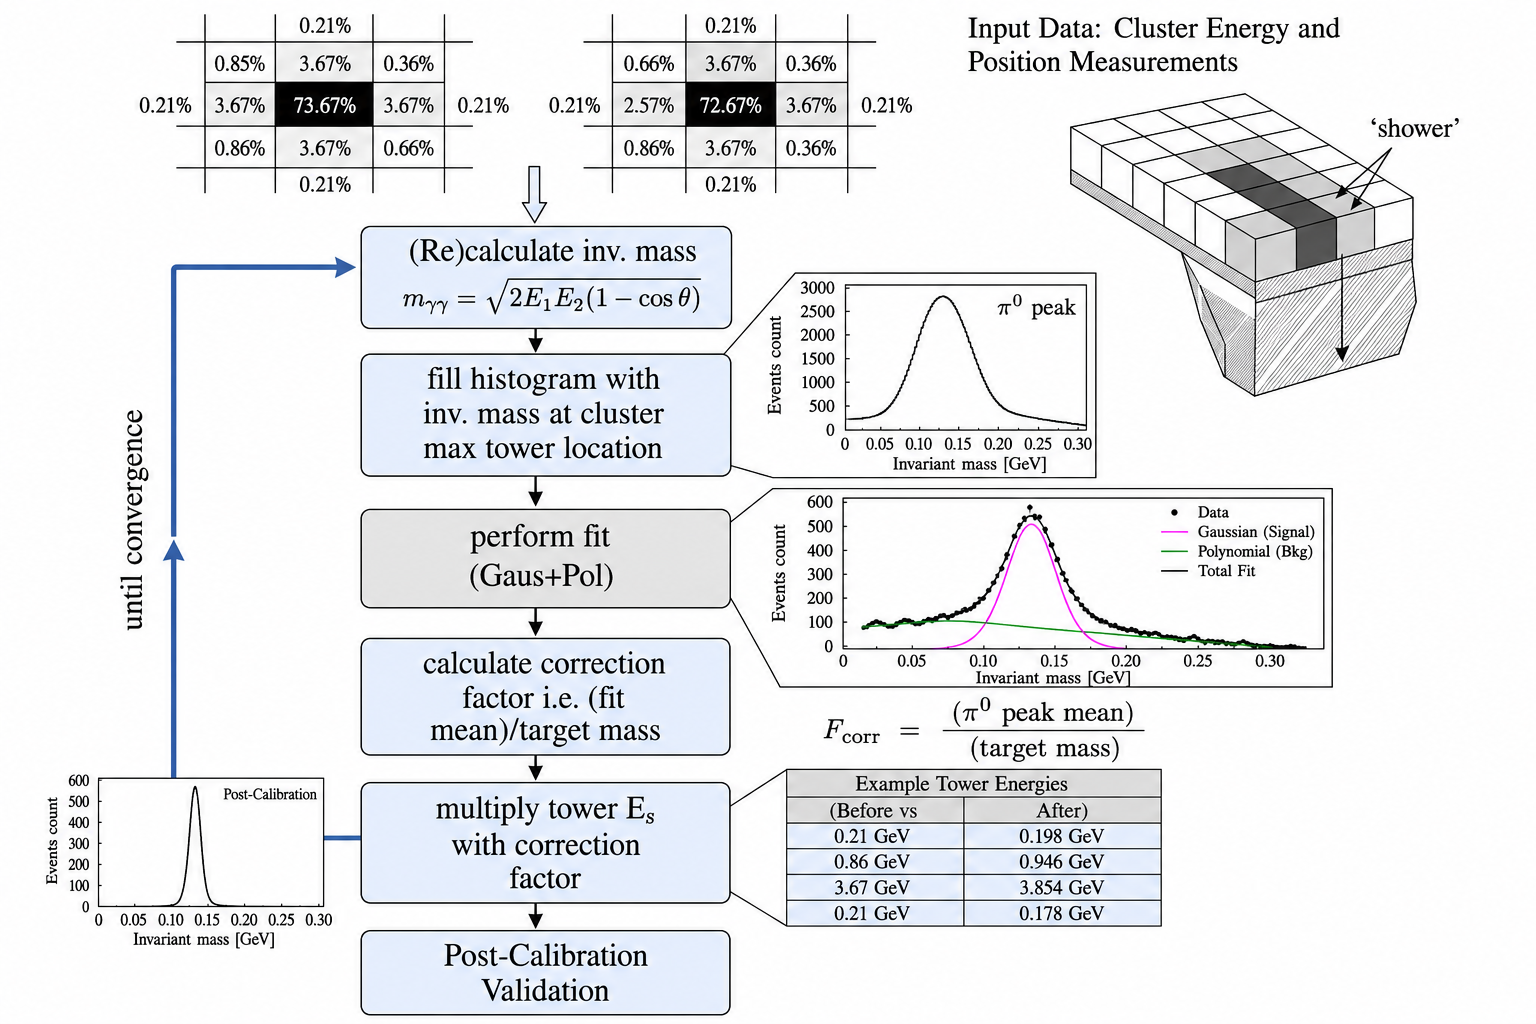
\includegraphics[width=0.95\textwidth,
    alt={Flowchart of the iterative EMCal calibration. Cluster energies and
         positions give the two-photon invariant mass; a histogram is filled at
         each cluster's maximum tower; the neutral-pion peak is fitted with a
         Gaussian plus polynomial; the correction factor, fit mean divided by
         the target mass, multiplies the tower energies; the loop repeats
         until convergence, followed by post-calibration
         validation.}]{Images/4_Plots/pi0_Calibration.png}
  %\includegraphics[width=0.8\textwidth]{Images/4_Plots/pi0_Calibration2.jpg}

  \caption{The schematic illustration of workflow for \ac{EMCal} calibration based on two photons invariant mass reconstruction. Photon cluster pairs are used to reconstruct the invariant mass and $\pi^0$ peak is fitted to ultimately determine tower-dependent energy correction factors. This procedure is repeated until the reconstructed $\pi^0$ mass converges to the target value. Image credit: Figure generated with combined assistance from Google Gemini and ChatGPT.}
  \label{fig:pi0_calib_workflow}
\end{figure}



\section{Implementing \texorpdfstring{$\pi^0$}{pi0} Calibration}

\ac{sPHENIX} took first data in 2023 and the $\pi^0$ calibration has been consistently implemented across different collision systems. During its operational lifetime, \ac{sPHENIX} has collected many dataset across $Au+Au$, $O+O$ and $p+p$ collisions. At the time of writing this dissertation, we have successfully implemented initial $\pi^0$ calibration on three datasets. 


%\begin{figure}[H]
\begin{figure}[tbh]
  \centering
  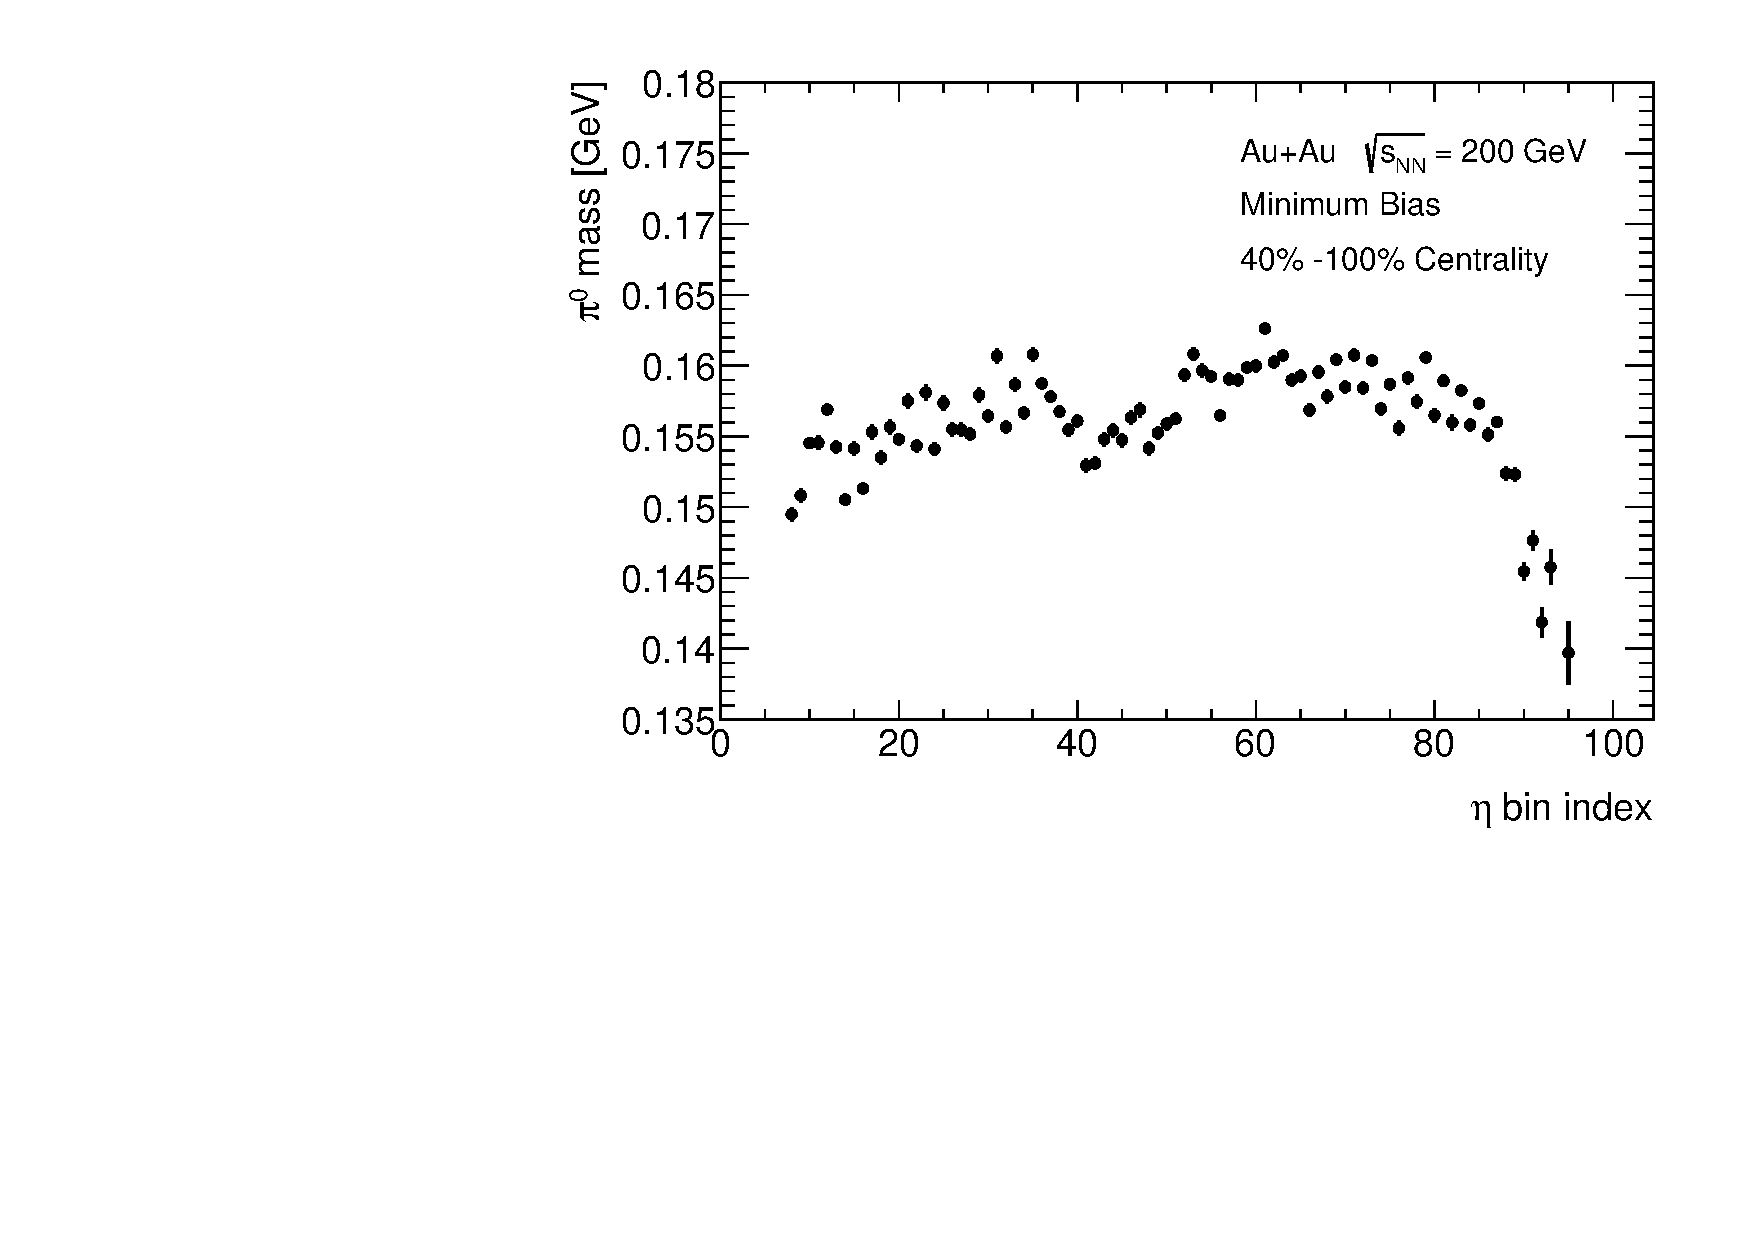
\includegraphics[width=0.95\textwidth,
    alt={Scatter plot of the reconstructed neutral-pion mass, about 0.15 to
         0.16 GeV, versus eta bin index from about 8 to 95, for Run 23 Au+Au
         minimum-bias collisions at 200 GeV with 40 to 100 percent
         centrality. The mass is roughly flat and drops toward 0.14 GeV at the
         highest bin indices.}]{Images/4_Plots/run23_AuAu_pi0_avg_mass.pdf}
  
  \caption{Reconstructed $\pi^{0}$ mass as a function of $\eta$ bin index in Run 23 $Au+Au$ data for first iteration while implementing absolute \ac{EMCal} calibration process. One unit of $\eta$ bin index corresponds to one tower along $\eta$ direction.}

  \label{fig:Run23Calib}
\end{figure}



As analysis presented in this dissertation was based on Run 24 \ac{pp} data, the calibration corresponding to this data set was used throughout the analysis. The final calibration value after six iteration of \ac{EMCal} calibration was used in our analysis. The tower by tower calibration was performed and those tower information were passes to ``clustering module'' to make cluster object. Those cluster objects were later used for our physics analysis.


